
\section{Representations}
\subsection{Classification}
% \begin{frame}{Purpose}
% 
\begin{tikzpicture}

% % always
\node (ds) at (5,0){};
\node (dsy) at (5,4){};
\node (dsx) at (10,0){};
\node (lab1) at (1,-1){\textbf{Chemical Space $C_f$}};
\foreach \x in {0,1,2}
		\foreach \y in {1,2,3}{
		\node[rectangle,fill=teal,minimum width = 0.05cm] (place\x\y) at (\x,\y){};}
% % two
\visible<2->{\node[draw,circle,very thick,red,minimum width = 0.5cm,label=right:{\color{red}$c_i$}] (ci) at (1,3){};}


% % three
\visible<3->{\node[circle, black,thick,minimum width = 2.7cm,minimum height = 2.7cm,path picture={\node at (path picture bounding box.center){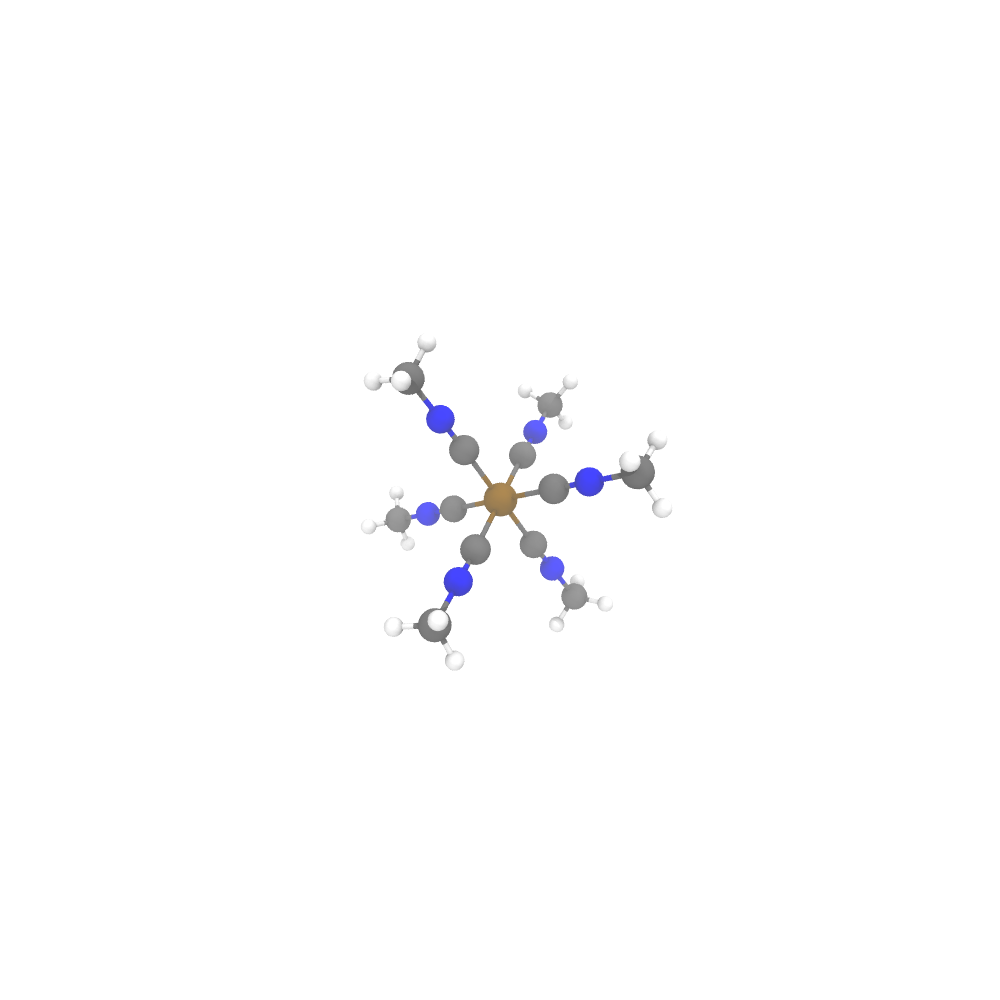
\includegraphics[width=7.5cm]{representations/images/misc}}; }] (Ap) at (3.45,3.75) {};}
\visible<3->{\node (A) at (3.45,3.75) {};}
\visible<3->{\node[draw,circle,very thick,red,minimum width = 2.75cm] (cic) at (3.45,3.75){};}
\visible<3->{\path[draw,red,dashed,very thick] (ci.north) edge node[below] {} (cic.north west);}
\visible<3->{\path[draw,red,dashed,very thick] (ci.south) edge node[below] {} (cic.south);}

% % four
\visible<4->{\path[draw,very thick] (ds.center) -- (dsx);}
\visible<4->{\path[draw,very thick] (ds.center) -- (dsy);}
\visible<4->{\node (lab1) at (7,-1){\textbf{Descriptor Space $\mathcal{X}\subset \mathbb{R}^{d}$}};}

% % five
\visible<5->{\node[circle, fill=black,minimum width =0.05cm,label=below:{$\mathbf{x}_i$}] (x) at (6,3) {};}
\visible<5->{\path[draw, thick,red] (cic.north east) edge[bend left,->] node[above] {} (x);}


% % six
\visible<6->{\node[circle, fill=black,minimum width =0.05cm,label=right:{$\mathbf{x}_{j}$}] (x3) at (8,1) {};}

% % seven
\visible<7->{\node[draw,circle,very thick,red,minimum width = 0.5cm,label=below:{\color{red}$c_j$}] (cj) at (2,1){};}
\visible<7->{\node[circle, black,thick,minimum width = 2.7cm,minimum height = 2.7cm,path picture={\node at (path picture bounding box.center){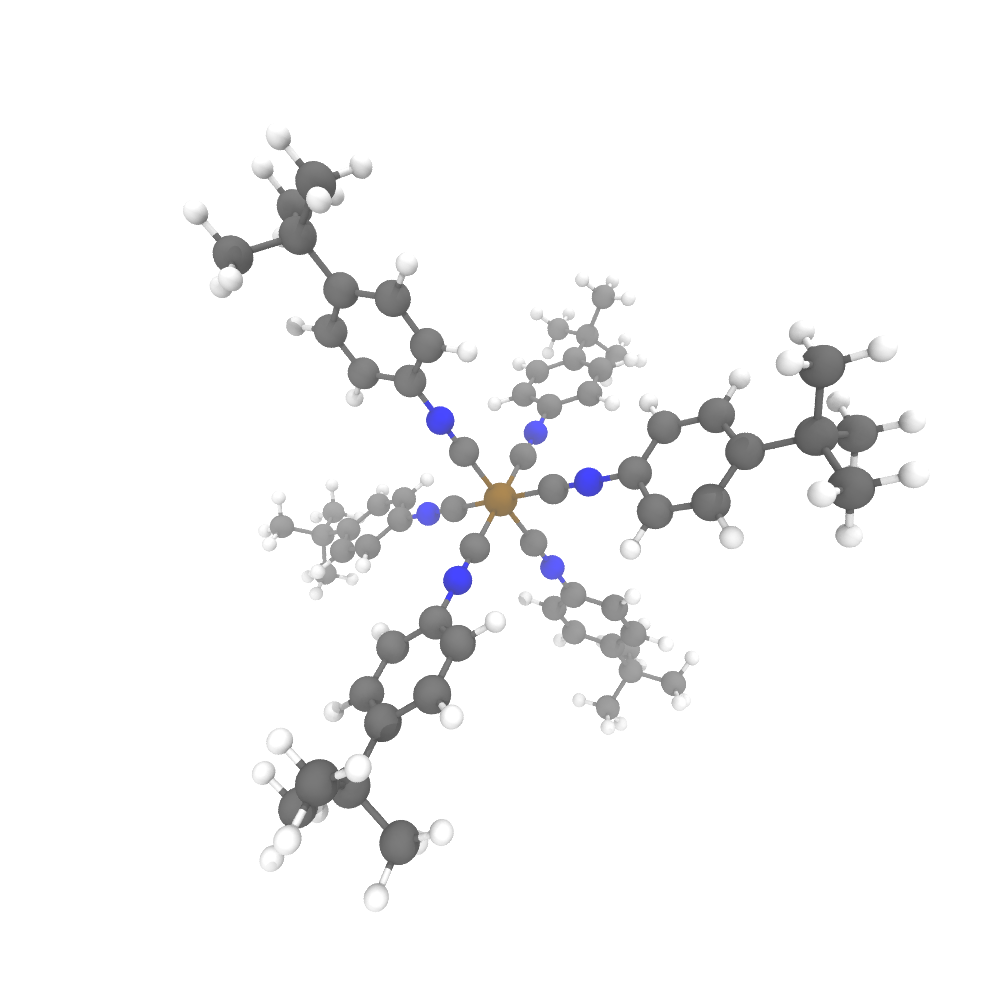
\includegraphics[width=3cm]{representations/images/pisc_trans}}; }] (Xp) at (4.2,0.75) {};}
\visible<7->{\node[draw,circle,very thick,red,minimum width = 2.75cm] (cicj) at (4.2,0.75){};}
\visible<7->{\path[draw,red,dashed,very thick] (cj.north) edge node[below] {} (cicj.north west);}
\visible<7->{\path[draw,red,dashed,very thick] (cj.south) edge node[below] {} (cicj.south west);}
\visible<7->{\path[draw, thick,red] (cicj.south east) edge[bend right,->] node[below] {} (x3);}

% % eight
\visible<8->{\path[draw,dashed,gray,very thick,|-|] (x) -- (x3);}
\visible<8->{\node[gray] (ddist) at (8,2){$d(\mathbf{x}_i,\mathbf{x}_j)$};}

% %
\visible<9->{\node[align=left] (gd) at (8.2,4) {Good descriptors: \\$\bullet$ cheap \\ $\bullet$ small as possible \\ $\bullet$ preserve similarity};}


\end{tikzpicture}

% \end{frame}
% \begin{frame}{Types of representation}

% \end{frame}
% \begin{frame}{Ad-hoc properties}

% \end{frame}
% \begin{frame}{Fingerprints and the low-information limit}

% \end{frame}
% \begin{frame}{Molecular graphs}

% \end{frame}
% \begin{frame}{Coulomb Matrices}
% \begin{center}
\begin{tikzpicture}[x=1cm,y=1cm]
%\pgfresetboundingbox
\draw[use as bounding box, anchor = north west,draw=none] (-5.5,-3.25) rectangle (5.5,3.25);
\clip (-5.5,-3.25) rectangle (5.5,3.25);
\only<1->{\node[anchor =north west] (text) at (-5.25,3.25){\begin{minipage}{10.0cm}
One family of 3D desciptors attempt to copy information used in quantum chemistry codes, e.g. Coulomb Matricies:\\
\scriptsize  Montavon, G. \textit{et al.}. Learning Invariant Representations of Molecules for Atomization Energy Prediction, NIPS 25, 2012 \normalsize
\begin{align*}
M_{I,J} = 
\begin{cases}
0.5Z_{I}^{2.4}& \text{for } I = J \\
\frac{Z_{I}Z_{J}}{|R_I-R_J|}&  \text{for } I \neq J
\end{cases}
\end{align*}		
\end{minipage}};}
\visible<1->{\node[anchor=east] (east) at (3.5,-1.5){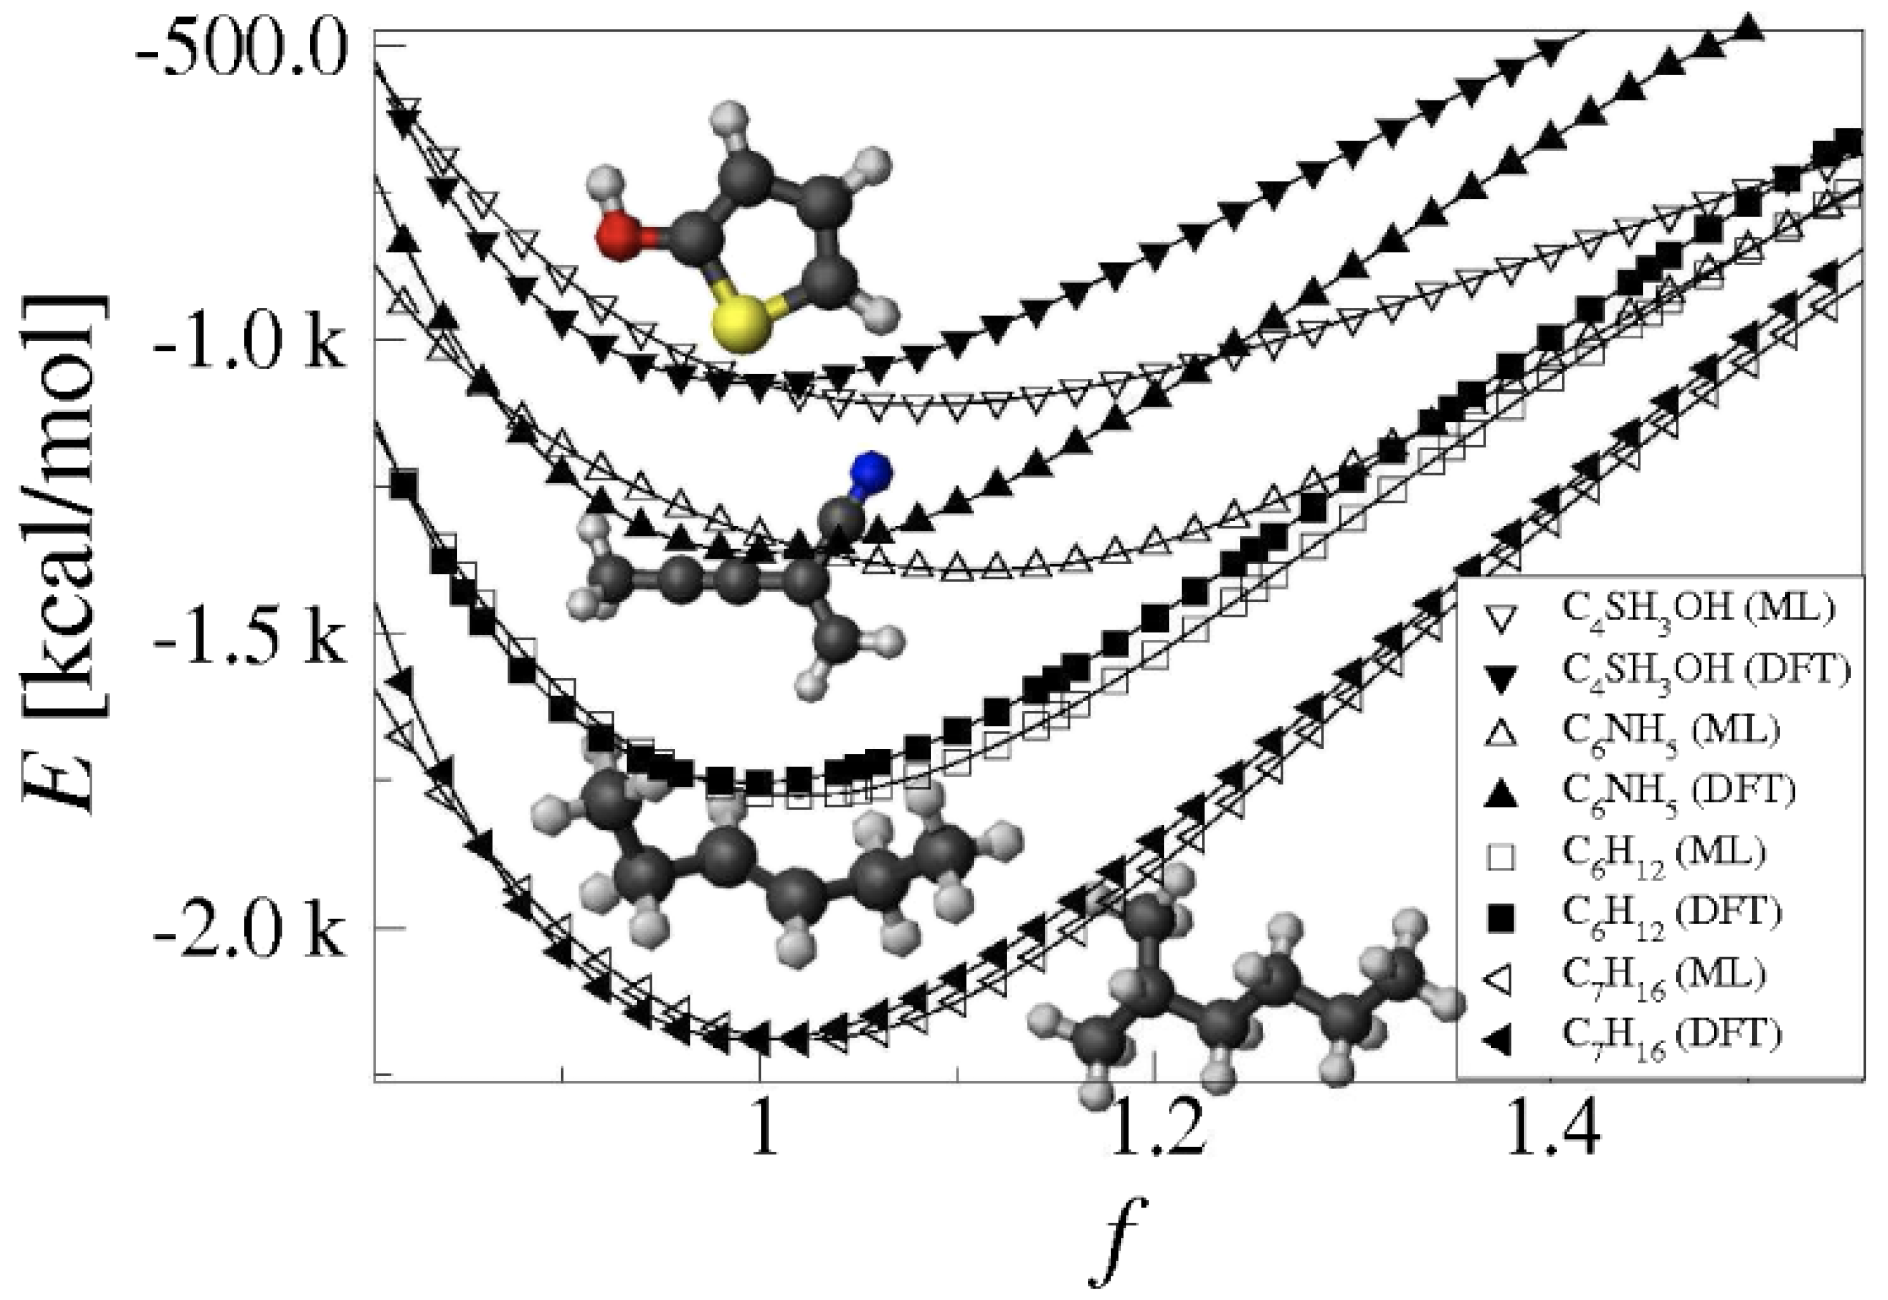
\includegraphics[width=3.5cm]{representations/images/coulomb_matrix_performance.png}};}
\visible<1->{\node[anchor=west] (figure) at (-4.5,-1.5){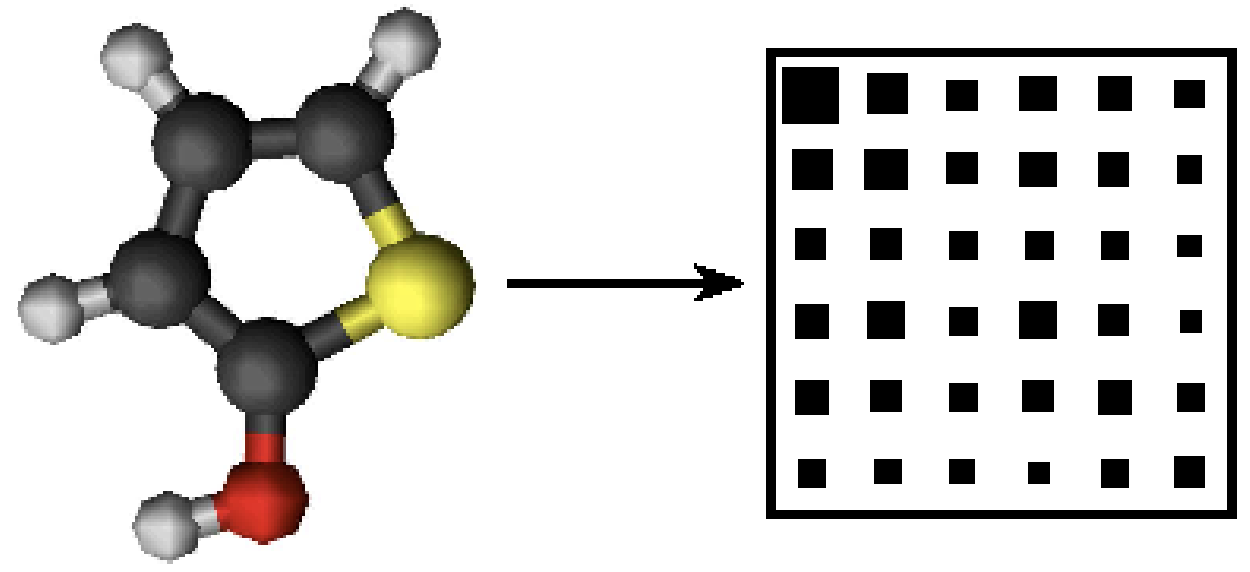
\includegraphics[width=3.5cm]{representations/images/coulomb_matrix.png}};}
\only<2->{\node[anchor = south] (text) at (1.5,-3.25){\begin{minipage}{10.0cm}
rotational and translational invariance
\end{minipage}};}
\end{tikzpicture}
\end{center}

% \end{frame}
\begin{frame}{HDAD and beyond-CM}
\begin{center}
	\begin{tikzpicture}[x=1cm,y=1cm]
	%\pgfresetboundingbox
	\draw[use as bounding box, anchor = north west,draw=none] (-5.5,-3.25) rectangle (5.5,3.25);
	\clip (-5.5,-3.25) rectangle (5.5,3.25);
	\only<1->{\node[anchor =north west] (text) at (-5.25,3.25){\begin{minipage}{10.0cm}
			Subsequent work adds descriptors derived from geometric parameters, i.e. bonds, angles, and dihedral angles:\\
			\scriptsize  Faber, F. \textit{et al.}. Prediction Errors of Molecular Machine Learning Models Lower than Hybrid DFT Error, \textit{J. Chem. Theory Comput.} 2017,  13, 11, 5255-5264 \normalsize
			\end{minipage}};}
	\visible<1->{\node[anchor=east] (east) at (3.5,-1.5){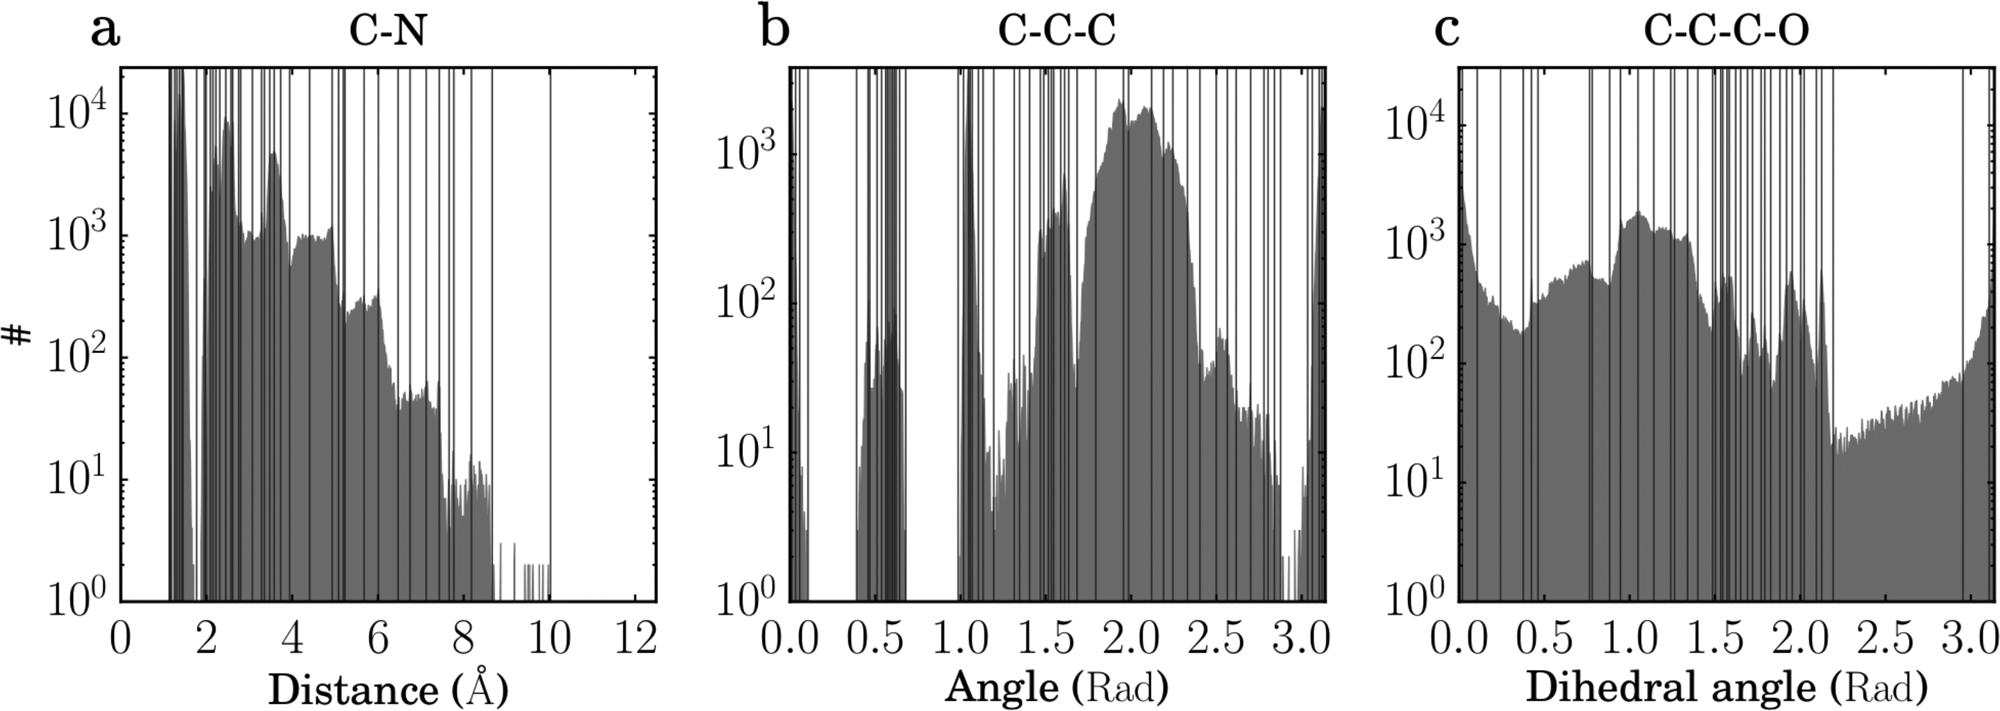
\includegraphics[width=3.5cm]{representations/images/HDAD}};}
	\visible<1->{\node[anchor=west] (figure) at (-4.5,-1.5){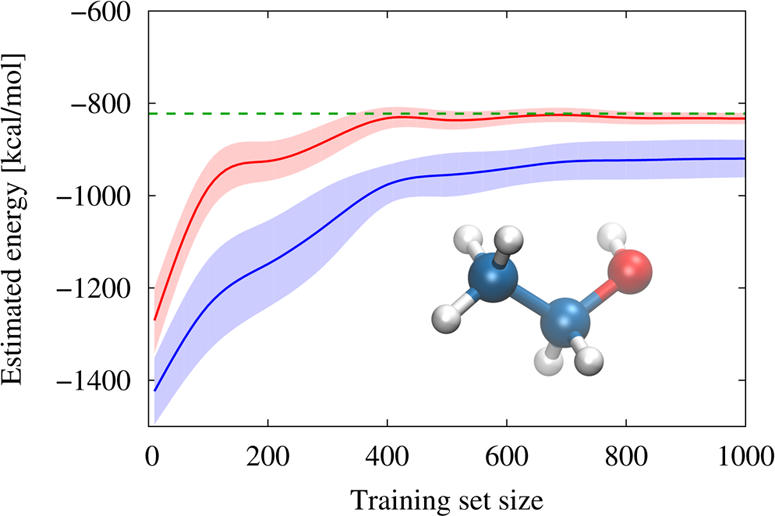
\includegraphics[width=3.5cm]{representations/images/HDAD_performance.jpg}};}
	\only<2->{\node[anchor = south] (text) at (1.5,-3.25){\begin{minipage}{10.0cm}
			add many, many more
			\end{minipage}};}
	\end{tikzpicture}
\end{center}

\end{frame}
% \subsection{Similarity}
% \begin{frame}{Why is one representation better than another?}
% two-complexes illustration 
% \end{frame}
% \begin{frame}{Why is one representation better than another?}
% also high learning rate and saturation issues
% \end{frame}

% \subsection{Feature selection}
% \begin{frame}{Feature selection}
% Why feature selection?
% \end{frame}
% \begin{frame}{Best subset selection}
% \begin{align*}
% w=\arg\min_{w\in \mathbb{d}}\left(\mathcal{L}\left( Xw \right) + K\left\Vert w \right\Vert _{0} \right) \: K\in\mathbb{N}_{0}
% \end{align*}
% \end{frame}
% \begin{frame}{LASSO and Elastic Net}
% special type of regularization -- need linear model
% understood as convex relaxation of best subset problem
% \end{frame}
% \begin{frame}{LASSO and Elastic Net}
% %
\begin{tikzpicture}[x=1cm,y=1cm]
\tikzstyle{line} = [draw, -latex', very thick]
\draw[use as bounding box, anchor = north west,draw,dashed,gray] (0,0) rectangle (5.5+5.5,3.25+3.25);
\clip (-0.15,-0.15) rectangle (11,6.5);
\node (ds) at (0,0){};
\node (dsy) at (0,2){};
\node (dsx) at (2,0){};
\node (dsxm) at (-2,0){};
\node (dsym) at (0,-2){};
\visible<1->{\path[line,very thick] (ds.center) -- (dsx);}
\visible<1->{\path[line,very thick] (ds.center) -- (dsy);}
\visible<1->{\path[line,very thick] (ds.center) -- (dsxm);}
\visible<1->{\path[line,very thick] (ds.center) -- (dsym);}
\node[circle,minimum width=2.82cm,draw, thick,fill=blue!20,opacity=0.5] (l2) at (0,0){};
\node[rectangle,minimum width=2.0cm,minimum height=2.0cm,draw, thick,rotate=45,fill=red,opacity=0.5] (l2) at (0,0){};
\end{tikzpicture}
% \end{frame}
